\documentclass[]{report}
\usepackage{tikz}
\newcommand{\inputtikz}[2]{%  
	\scalebox{#1}{\input{#2}}  
}
\usepackage[english]{babel}
\usepackage[utf8x]{inputenc}
\usepackage{amsmath}
\usepackage{graphicx}
\usepackage[colorinlistoftodos]{todonotes}
\usepackage{listings}
\usepackage{color}
\usepackage{amsmath}
\usepackage{amsfonts}
\usepackage{mathtools}
\usepackage{graphicx}
\usepackage{caption}
\definecolor{dkgreen}{rgb}{0,0.6,0}
\definecolor{gray}{rgb}{0.5,0.5,0.5}
\definecolor{mauve}{rgb}{0.58,0,0.82}
%opening

\begin{document}
	
\begin{titlepage}
	
	\newcommand{\HRule}{\rule{\linewidth}{0.5mm}} 
	
	\center 
	
	\textsc{\LARGE Université de Technologie de Compiegne}\\[1.5cm]
	\textsc{\Large SY19}\\[0.5cm] 
	\textsc{\large Machine Learning}\\[0.5cm]
		
	\HRule \\[0.4cm]
	{ \huge \bfseries First Assignment}\\[0.4cm] 
	\HRule \\[1.5cm]
		
	\begin{minipage}{0.4\textwidth}
		\begin{flushleft} \large
			Aladin \textsc{TALEB} 
		\end{flushleft}
	\end{minipage}
	~
	\begin{minipage}{0.4\textwidth}
		\begin{flushright} \large
			Zineb \textsc{SLAM} 
		\end{flushright}
	\end{minipage}\\[2cm]

	{\large \today}\\[2cm] 

	
\includegraphics[width=40mm]{Figures/utc.jpg}\\ % 

	\vfill
	
\end{titlepage}

\lstset{frame=tb,
	language=R,
	aboveskip=3mm,
	belowskip=3mm,
	showstringspaces=false,
	framexleftmargin=5mm,
	columns= fixed,
	numbers = left,
	basicstyle={\small\ttfamily},	
	numberstyle=\tiny\color{gray},
	keywordstyle=\color{blue},
	commentstyle=\color{dkgreen},
	stringstyle=\color{mauve},
	breaklines=true,
	breakatwhitespace=true,
	tabsize=3
}

	

\begin{abstract}
	
	
	
This report is an assignment for the course SY19 : Machine Learning. It is focused on two exercises : a regression problem (Chapter I) and classification problem (Chapter II) . In each part, we will describe the methodology we used to build the best model for each dataset.\\
The content presented in this report is the result of the theoretical and practical courses of SY19 taught by Thierry Denoeux and a literature review. We put on a side note that we both have not followed SY09, and only one of us has already done SY02, which prevented us to go deeper in the explanations and analysis sometimes but we made sure to make researches every time it was needed.

\end{abstract}


\tableofcontents

\newpage
\section{Abbreviations}
\begin{center}
\begin{tabular}{l r}
	MSE & Mean Squared Error \\
	RSE & Resiual Standard Error\\ 
	RSS & Residual Sum of Squares \\
	AIC & Akaike information criterion \\
	BIC & Bayesian information criterion \\
	$R^{2}$ & Adjusted $R^{2}$ \\
	LR & Linear Regression \\
	CV & Cross Validation \\
	LOOCV & Leave One Out Cross Validation \\
\end{tabular}
\end{center}



\chapter{Breast Cancer Recurring Time}

\section{Context}
This part aims to build the best model to predict the recurring time of breast cancer based on about 30 features computed from a breast mass.  This regression problem will take advantage of a given dataset describing about 200 patient cases.

\section{Dataset Description}
The very first step of our method consists in taking a look at the raw dataset to get precious hints on how each feature contributes to the recurring time. The dataset comprises 194 patient cases, each of which is described through 32 features and the cancer recurring time \texttt{Time} that we have to predict.

\subsection{Time}
Let's first describe the distribution of the variable \texttt{Time}. To do so, we can use the R functions \texttt{boxplot} (figure \ref{fig:time_boxplot}) and \texttt{hist} (figure \ref{fig:time_hist}). According to these figures, our dataset mostly represents short reappearing times (lower than 40), and there are very few patients whose variable \texttt{Time} is higher than 80. However, we do not know if this distribution is also representative of the whole population. If this is is the case, our model should be able to work on other datasets, if not, our model will be biaised.

\begin{figure}[!hb]
	\centering
	\inputtikz{0.5}{Figures/time_boxplot.tex}
	\caption{Box Plot}
	\label{fig:time_boxplot}
\end{figure}

\begin{figure}[!h]
	\centering
	\inputtikz{0.5}{Figures/time_hist.tex}
	\caption{Histogram}
	\label{fig:time_hist}
\end{figure}


\subsection{Features Description}
Each patient is represented with a set of 32 features extracted and computed from a digitized image of a breast mass. The data description we were given does not specify the units, but we do not need them for the following analysis. Here are the 32 features we are provided with:  
\begin{itemize}
	\item Lymph Node Status
	
	\item Mean, Standard Error and Mean of the three largest values (also called "Worst") of 
	\begin{itemize}
		\item Radius
		\item Texture
		\item Perimeter
		\item Area
		\item Smoothness
		\item Compactness
		\item Concavity
		\item Concave points
		\item Symmetry
		\item Fractal dimension
	\end{itemize}
	
	\item Tumor Size
\end{itemize}

\subsubsection{Feature Correlation}
Based on the definition of the parameters described above, we already know that many features are correlated. For instance : 
\begin{itemize}
	\item The mean of each parameters is smaller than the "worst" value;
	\item The radius, the perimeter and the area are most likely to be linked together;
	\item The compactness can be computed with the perimeter and the area thanks to the given formula : $Compactness = \frac{perimeter^2}{area - 1}$
\end{itemize}

These dependent features might be a cause of model low performance.

\subsection{Data Relevance}
We should first check that every patient is relevant to our study, in other words, that there is no abnormal observation in the dataset. Cook's Distance is an interesting measure to verify this important criteria, it can be computed after a simple Linear Regression.

Cook's distance aims to study the influence of each observation on the regression coefficient estimates. To do so, this method uses a straight-forward approach that consists in computing the difference between the original coefficient estimates $\hat{\beta}$ and the coefficient estimates without taking into account the $i$-th observation $\hat{\beta}_{(-i)}$. The difference is then normalized using the number of parameters and the standard deviation estimate. A value higher than 1 often indicates an outlier that should be removed from the dataset.

In R, we can use the following code to compute and plot the Cook's distance of each observation :

\begin{lstlisting}
linreg = lm(Time ~ ., data=data_set)
cooks.distance(linreg)
\end{lstlisting} 

\begin{figure}[!h]
	\centering
	\inputtikz{0.5}{Figures/cooks_distance.tex}
	\caption{Cook's Distance}
	\label{fig:cook_distance}
\end{figure}

According to this plot (figure \ref{fig:cook_distance}), no observation is located beyond the critical Cook's boundary of 1. This means that we can potentially use each and every patient case of our dataset to build our regression model. 

\subsection{Relation between "feature" and "time"}
In this section, we will take a first look at the relationship between the variable \texttt{Time} and the features used to describe a patient case. 

A first way to do it is to separately plot \texttt{Time} against each feature. An example of such plot is shown in figure \ref{fig:time_feature_ex1}. Unfortunately, most plots picture very scattered points that do not seem to follow any specific model. The variance is so significant that we cannot even estimate the type of function that links a feature and the variable \texttt{Time} together. It could be a simple linear model with a high variance that we may be able to estimate, or more complex models with non-linearities and feature correlations.

\begin{figure}[!h]
	\centering
	\inputtikz{0.5}{Figures/time_feature_ex1.tex}
	\caption{Plot of \texttt{Time} against \texttt{Texture Mean} }
	\label{fig:time_feature_ex1}
\end{figure}

To have better clues on the type of model we should be dealing with, we can draw a QQ-Plot that plots the Studentized Residuals against the quantiles. 

In R, we can use the library \texttt{car} to easily draw the QQ-Plot (figure \ref{fig:qq_plot}) :
\begin{lstlisting}
library(car)
qqPlot(linreg, main="QQ Plot")
\end{lstlisting}

\begin{figure}[!hb]
	\centering
	\inputtikz{0.5}{Figures/qq_plot.tex}
	\caption{QQ-Plot}
	\label{fig:qq_plot}
\end{figure}

The bottom tail of the QQ-Plot seems to deviate from the linear line, which is a sign of the error's non-normality. This may mean that the error does not follow a normal model, or that the model is actually non-linear.

\begin{figure}[!hb]
	\centering
	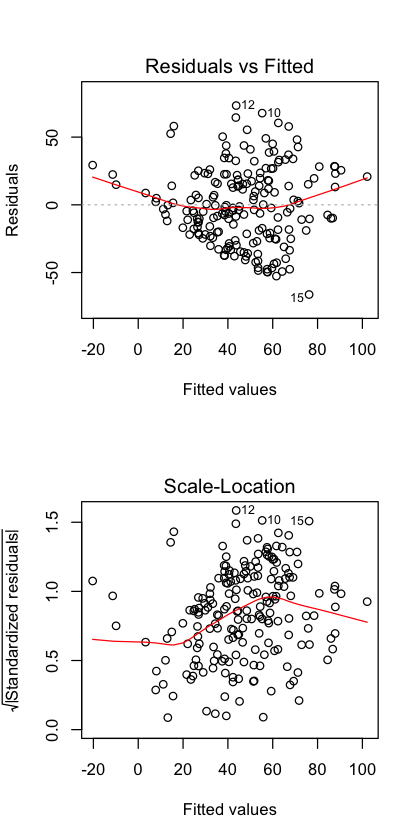
\includegraphics[width=0.5\linewidth]{Figures/fitted_value_plots}
	\caption{}
	\label{fig:fitted_value_plots}
\end{figure}

We can also analyze the Residuals-Fitted plot and the Scale-Location plot to get a better understanding on the model. To do, we can simply apply the function \texttt{plot} on the linear model (figure \ref{fig:fitted_value_plots}). It turns out that both plots show non-normal scatters of the residuals. In particular, the points displayed in the Residuals-Fitted plot seem to follow a fan shape. This is a sign of a non-constant variance, also called heteroscedasticity.

\section{Measures to Compare Models}
Before building any model, we have to properly define the measures we will use later to compare their performance. 

\subsection{Some Measures}
A first way to assess the performance of a model $F$ is to compute the Mean Squared Error (MSE). Let $\hat{Time}$ be the estimate of the variable $Time$ using the model $F$. MSE is defined as :
$$MSE(F) =  mean_i(Time_i - \hat{Time}_i)^2$$

We can also use adjusted $R^2$ score.

\subsection{Data Split}
These measures should not be applied on a set whose data was also used to train the model. Indeed, this would include a biais that might distort our conclusions. To cope with this problem, we have to split the dataset into two disjointed sets : 
\begin{itemize}
	\item Training Set : About 66\% of the dataset dedicated to the model fitting;
	\item Test Set : The remaining 34\% only used at the end to provide some kind of objective measure of the model performance.
\end{itemize} 

\begin{lstlisting}
n = dim(data_set)[1]
train_id = sample(1:n, n * 2/3)

train_set = data_set[train_id,]
train_set.x = train_set[,-33]
train_set.y = train_set[,33]

test_set = data_set[-train_id,]
test_set.x = test_set[,-33]
test_set.y = test_set[,33]
\end{lstlisting}

Once this data split is done, we can finally dive into the model building.

\section{K-nearest neighbors (KNN)}
We start our analysis with a very simple model called the KNN.
Given a positive integer $k$ and a test observation. The KNN model first identifies the k closest points to each point of the test observation then it estimates the response using the average of the k closest training responses.\\ 

\subsection{Knn Model}
The KNN model in R is done by calling the function \texttt{reg} of the package \texttt{knn}. As we will see in the following sections, For most prediction algorithms, we first have to build the prediction model on the training data, and then use the model to test our predictions. However, the KNN function does both in a single step.\\ 
In order to find the best $k$ we set a maximum number of neighbors to be considered (in our model it is 120), then we calculate the MSE for each $k$ which is the mean of the squared difference between the real value of \texttt{Time} and the predicted one. All the steps are detailed in the code below.

\subsubsection{Model Implementation}
\begin{lstlisting}
library(FNN)
k_max = 120;
MSE = rep(0,k_max)

for( k in 1:k_max)
{
model.knn = knn.reg(train=train_set.x, test=test_set.x, y=train_set.y, k=k)
MSE[k] = mean((test_set.y - model.knn$pred)^2)
}

model.knn.best.k = which.min(MSE)
model.knn.best.MSE = MSE[model.knn.best.k] 
\end{lstlisting}

The graph below (figure \ref{fig:knn_train}) shows the \textbf{ MSE} plotted against the values of $k$ in a range from 0 to 120. Graphically we notice that a minimum is reached between 10 and 20.

\begin{center}	
	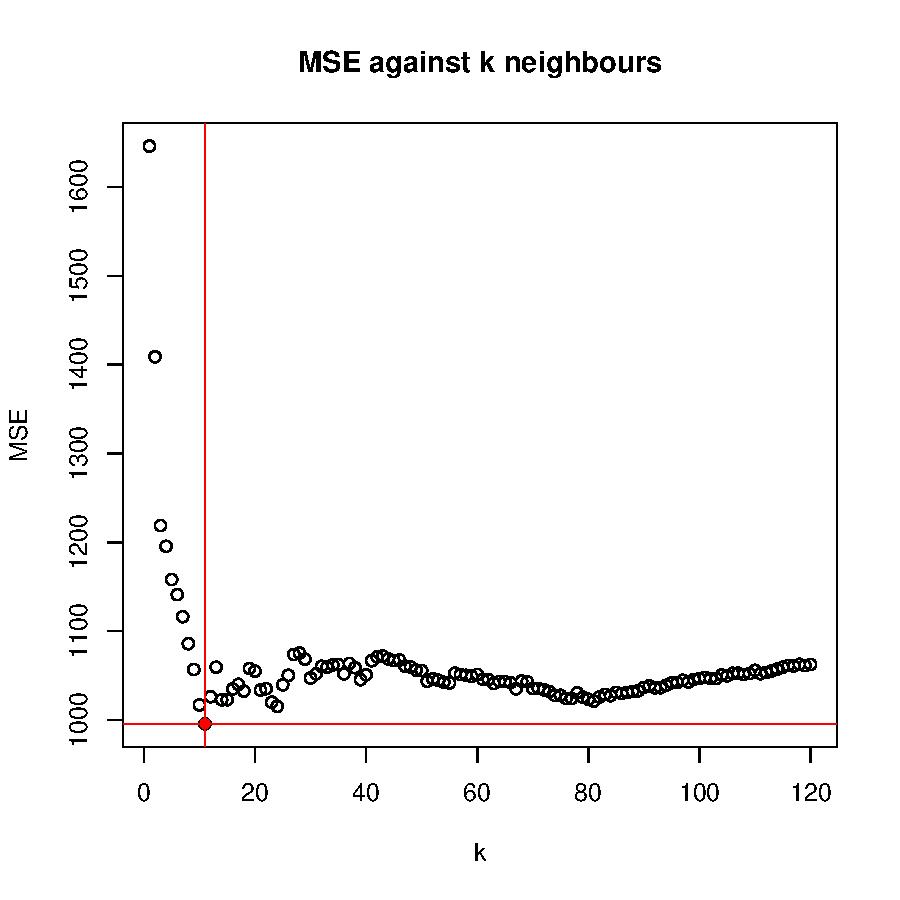
\includegraphics[width=0.9\linewidth]{Figures/knn_test.pdf}
	\captionof{figure}{MSE against K neighbours \textit{(minimum in red)}}
	\label{fig:knn_train}
\end{center}

We are looking for the k neighbors that has the smallest MSE so we use the function \texttt{which.min} that returns the index of the minimum value of MSE.\\

\begin{center} 
	model.knn.best.k   = 11 \\
	model.knn.best.MSE = 1060.46
\end{center}

Now that we have the $k$ that minimizes the MSE we call KNN algorithm with this best $k$ and plot the predicted values against the real values as the residuals. The corresponding code is shown below:

\begin{lstlisting}
model.knn.best = knn.reg(train=train_set.x, test=test_set.x, y=train_set.y, k=model.knn.best.k)
plot(test_set.y,model.knn.best$pred, xlab='y', ylab='y-hat', main='y-hat (Predicted) against y')
abline(0,1, col='red')

model.knn.best.residuals = test_set.y - model.knn.best$pred

hist(model.knn.best.residuals, freq=FALSE, main="Distribution of Residuals in Knn best case")
residuals.mean = mean(model.knn.best.residuals)
residuals.stdev = sqrt(var(model.knn.best.residuals))
curve(dnorm(x, mean=residuals.mean, sd=residuals.stdev), col="darkblue", lwd=2, add=TRUE, yaxt="n")
\end{lstlisting}

The red line is the function $y=x$; so further are the points from this line the further are the predicted values ($\hat{y}$) from the real one ($y$).

\begin{center}
	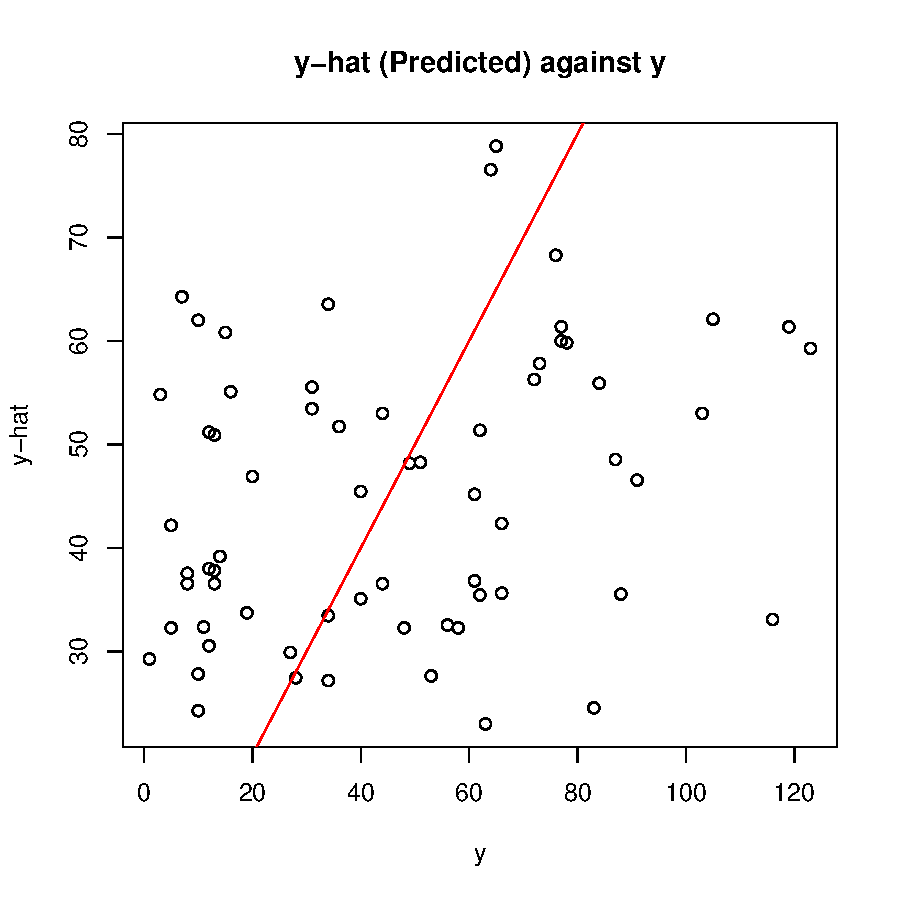
\includegraphics[width=0.9\linewidth]{Figures/knn_predicted_test.pdf}
	\captionof{figure}{Predicted values against the real values}
	\label{fig:knn_predicted_test}
\end{center}

\begin{center}
	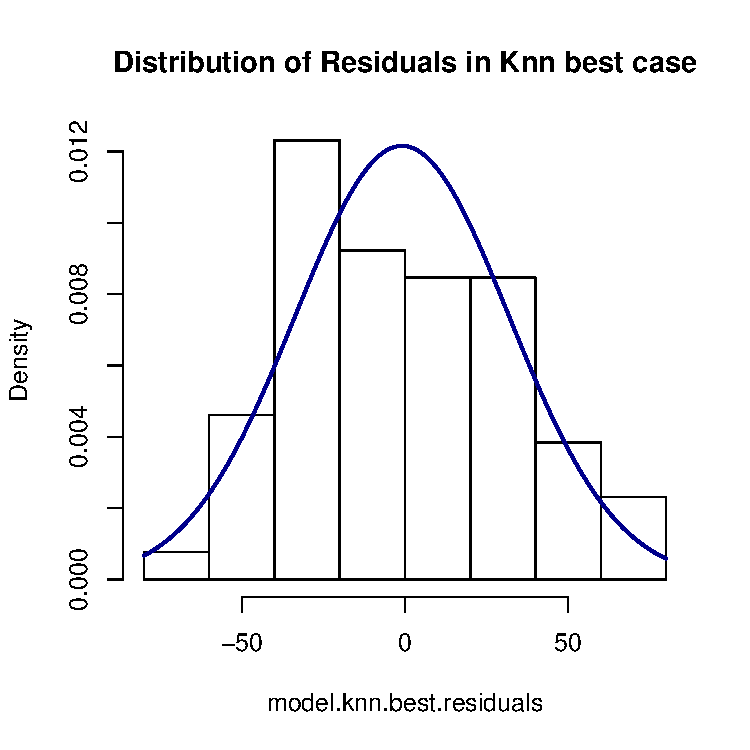
\includegraphics[width=0.9\linewidth]{Figures/knn_predicted_test_residuals.pdf}
	\captionof{figure}{Distribution of Residuals in Knn best case}
	\label{fig:knn_predicted_test_residuals}
\end{center}


\subsubsection{Model Analysis}

We notice that the predicted {$\hat{y}$} diverge a lot from the real values $y$. We expected those results since the MSE is around 967 which is quite high. 

This approach of finding the best $k$ was quite optimistic. Actually we tried finding the best $k$ while minimizing the MSE in \textbf{the test data}. Therefore the model is very specific to our test data which yields to a high bias. The solution is to find the best $k$ among the \textbf{training data} and then use the best $k$ in the test data. \\ To find the best \textbf{unbiased} $k$ number of neighbors k we use the method of cross validation on the train data then we predict the response on the test. 

\subsection{The Validation Set Approach}
There are two main methods in cross validation: \textbf{the validation set approc}h and the \textbf{cross validation leave one out (LOOCV)} which is a particular case of the  \textbf{K-fold cross validation}. As we do not have that much observations (n=198) we can afford the computation of cross validation leave one out, but before we will argument our choice.\\

\subsubsection{Cross Validation}
The cross validation approach is based on dividing the provided data in 2 sets: a training set and a validation set. The model is fit on the training set, then the fitted model is used to predict responses of observations in the validation set. We validate our model using the best MSE.

\subsubsection{Leave-One-Out Cross-Validation}
Like the cross validation the LOOCV involves splitting the set of observations in two parts. The main difference is that we have a single observation $(x_1, y_1)$ in the test data and the $n-1$ remaining is used for the train data. The MSE in this case is $MSE_1 =(y_1 - \hat{y})^{2}$. This provides an unbiased estimate for the test error since the size of the train model is approximately the one of all the data of the observation. However it is highly variable as it is based in one observation. The LOOCV repeats the procedure n times fitting each time a different set of observations. The LOOCV test MSE is computed with calculating the average of the n test error estimates.

\begin{center}
	$$CV_{(n)} = \frac{1}{n} \sum_{i=1}^{n} MSE_{i} $$
\end{center}

The LOOCV will always give the same results in contrast to the CV that depends on the randomness of how the data are split. Furthermore as it was stated before the CV runs the train approach on around the half of the size of the original data while the LOOCV repeats the validation set approach n times using n-1 observations. Hence the LOOCV yields to a not overestimated test error rate compared to the validation set approach. The only disadvantage of the LOOCV is it is computation time which can be very time consuming n is large.\\

An alternative to LOOCV that has a smaller computation time is k-Fold Cross Validation. This approach is based on dividing the training observations on $k$ groups, each time one group will be considered as the test set and the $k-1$ left as the training set. Therefore the CV becomes:

\begin{center}
	$$CV_{(k)} = \frac{1}{k} \sum_{i=1}^{k} MSE_{i} $$
\end{center}

We can see that the k-Fold Cross-Validation fits the model $k$ times instead of $n$, which reduces considerably the computation time. Our original data has only 198 observations, we can then afford the computation of the LOOCV. \\

\subsubsection{Model implementation}

\begin{lstlisting}
library("kknn")
model.kknn = train.kknn(Time ~., data= train_set, kmax = 30, ks = NULL, distance = 2, kernel = "optimal")
model.kknn.best.k = model.kknn$best.parameters$k
\end{lstlisting}

After deducting the best k neighbors from the model we use it on the test observations to predict the values of Time. 
We then compute the MSE and plot the predicted values $\hat{y}$ against the real ones \textit{y}.

\begin{lstlisting}
library("kknn")
model.kknn = train.kknn(Time ~., data= train_set, kmax = 30, ks = NULL, distance = 2, kernel = "optimal")
model.kknn.best.k = model.kknn$best.parameters$k

model.kknn.best = knn.reg(train=train_set.x, test=test_set.x, y=train_set.y, k=model.kknn.best.k)
plot(test_set.y, model.kknn.best$pred, xlab='y', ylab='prediction')
abline(0,1, col='red')

residuals = test_set.y - model.kknn.best$pred
errors = residuals^2
model.kknn.best.MSE = mean(errors)

hist(residuals, freq=FALSE, main="Distribution of Residuals in Knn LOOCV best case")
residuals.mean = mean(residuals)
residuals.stdev = sqrt(var(residuals))
curve(dnorm(x, mean=residuals.mean, sd=residuals.stdev), col="darkblue", lwd=2, add=TRUE, yaxt="n")
\end{lstlisting}

\begin{center} 
	model.kknn.best.k  = 30 \\
	model.kknn.best.MSE = 1146.05
\end{center}

We run a the same plot again with the predicted reponses against the real ones \ref{fig:knn_predicted_LOOCV} and the histogram of the residuals \ref{fig:knn_predicted_residuals_LOOCV}.
.
\begin{center}
	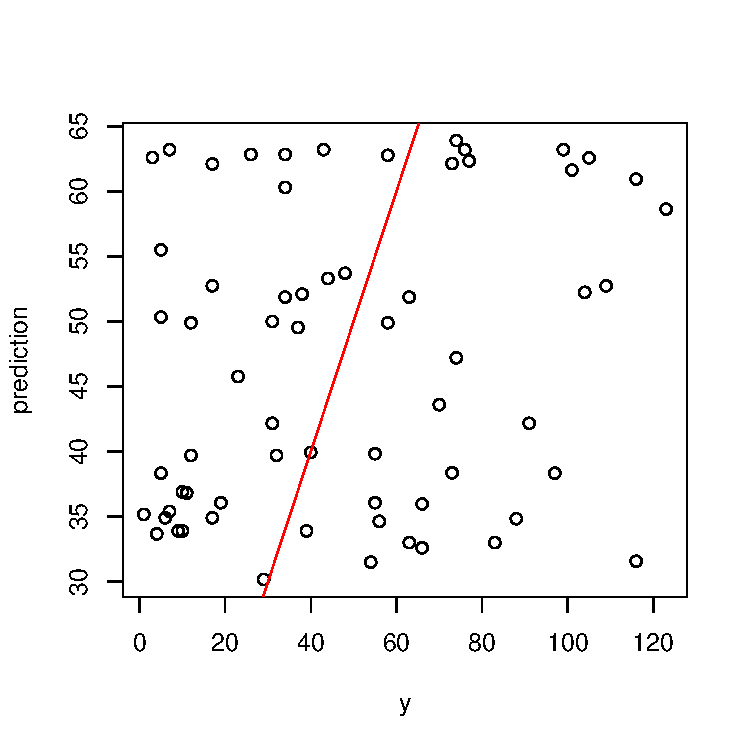
\includegraphics[width=0.8\linewidth]{Figures/knn_predicted_LOOCV.pdf}
	\captionof{figure}{Predicted values against Real values with LOOCV}
	\label{fig:knn_predicted_LOOCV}
\end{center}

\begin{center}
	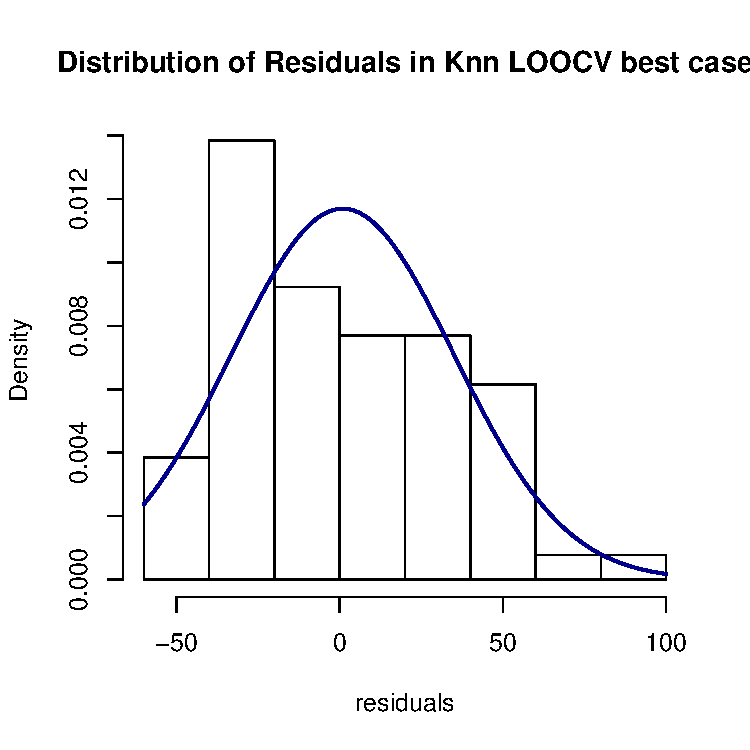
\includegraphics[width=0.8\linewidth]{Figures/knn_predicted_LOOCV_residuals.pdf}
	\captionof{figure}{Distribution of Residuals in Knn with LOOCV}
	\label{fig:knn_predicted_residuals_LOOCV}
\end{center}



\subsubsection{Model Analysis}
One might argue that the prediction was not improved with the LOOCV since the test MSE obtained is higher that the MSE we obtained when we computed using the test set directly. However this result was expected since in the first approach we run our knn directly on the test so we underestimated the MSE, in other words the first MSE is specific to that test set of data (biased), in contrast to our the LOOCV model. In other words, in general the $k=30$ will guarantee a smaller MSE than the $k=11$ on any test observation.
The LOOCV has also an advantage over the first approach because it will always give the same result of best k.

\section{Simple Linear Regression}
\subsection{Idea}
Our next attempt consists in using the same linear model we used in the feature analysis section. This model takes advantage of the simple assumption that \texttt{Time} depends on the other features in a linear way. A linear regression model has the following form :
$$
Y = \beta_0 + \sum_{i = 1}^{p} \beta_i X_i
$$
The regression coefficients $\beta_i$ are choosen so that they minimize the MSE. Both analytical and optimization methods (Gradient Descent, Stochastical Gradient Descent, ...) can be used to find the best coefficient estimates.

To build the model in R, we can use the function \texttt{lm} :
\begin{lstlisting}
model.linreg = lm(Time ~ ., data=train_set)
\end{lstlisting}

\subsection{Model Performance}
This model has a MSE approximatively equal to 1285. The raw residuals distribution is pictured on figure \ref{fig:linreg_hist}, it shows a very spread out distribution that should be improved.

\begin{figure}[!h]
	\centering
	\inputtikz{0.5}{Figures/linreg_hist.tex}
	\caption{}
	\label{fig:linreg_hist}
\end{figure}

\begin{figure}[!h]
	\centering
	\inputtikz{0.5}{Figures/linreg_predicted.tex}
	\caption{}
	\label{fig:linreg_predicted}
\end{figure}

\section{Linear Regression with Features Selection}
\subsection{Idea}
A simple method to improve the performance of the previous Linear Regression is to select a subset of features that better describes the distribution of \texttt{Time}.

Once the simple linear model is fitted, we can use the function \texttt{summary} to display the value of each coefficient.
\begin{verbatim}
Coefficients:
Estimate Std. Error t value Pr(>|t|)  
(Intercept)              5.722e+01  1.587e+02   0.361   0.7191  
Lymph_node              -1.752e-01  7.034e-01  -0.249   0.8038  
radius_mean              3.001e+01  4.445e+01   0.675   0.5012  
texture_mean            -3.913e-01  2.043e+00  -0.192   0.8485  
perimeter_mean          -3.794e+00  6.651e+00  -0.570   0.5697  
area_mean               -1.328e-01  1.354e-01  -0.981   0.3291  
smoothness_mean         -7.124e+02  9.050e+02  -0.787   0.4331  
compactness_mean        -8.767e+01  3.554e+02  -0.247   0.8057  
concavity_mean          -2.654e+02  2.728e+02  -0.973   0.3332  
concave_points_mean      1.236e+03  5.911e+02   2.090   0.0392 *
symmetry_mean           -3.199e+01  2.647e+02  -0.121   0.9041  
fractal_dimension_mean   1.818e+03  1.666e+03   1.091   0.2781  
radius_se               -2.897e+01  9.953e+01  -0.291   0.7716  
texture_se              -1.784e+00  1.246e+01  -0.143   0.8865  
perimeter_se             8.817e+00  1.289e+01   0.684   0.4955  
area_se                 -3.871e-01  4.212e-01  -0.919   0.3604  
smoothness_se            2.987e+03  2.535e+03   1.178   0.2415  
compactness_se           7.135e+02  7.864e+02   0.907   0.3665  
concavity_se             3.798e+02  7.170e+02   0.530   0.5975  
concave_points_se       -7.782e+02  1.450e+03  -0.537   0.5926  
symmetry_se             -1.239e+03  7.861e+02  -1.576   0.1182  
fractal_dimension_se    -5.979e+03  6.280e+03  -0.952   0.3434  
radius_worst             9.300e-01  1.367e+01   0.068   0.9459  
texture_worst           -1.307e+00  1.964e+00  -0.666   0.5072  
perimeter_worst         -1.026e+00  1.449e+00  -0.708   0.4805  
area_worst               8.705e-02  7.021e-02   1.240   0.2181  
smoothness_worst        -3.761e+02  4.088e+02  -0.920   0.3599  
compactness_worst       -7.031e+01  9.964e+01  -0.706   0.4821  
concavity_worst         -3.011e+01  7.311e+01  -0.412   0.6814  
concave_points_worst    -2.181e+02  2.345e+02  -0.930   0.3546  
symmetry_worst           1.586e+02  1.425e+02   1.113   0.2687  
fractal_dimension_worst  1.028e+03  7.100e+02   1.448   0.1509  
Tumor_size              -1.188e+00  1.915e+00  -0.620   0.5364  
\end{verbatim}

The last column contains the P-value of each coefficient, which is a measure to test the hypothesis that this particular coefficient is null. A P-value lower than 5\% allows us to conclude that the coefficient is not equal to zero. In our case, the feature \texttt{concavity\_points\_mean} is not null, but we cannot make such assumptions for the other parameters. Therefore, we are not able to select a subset of interesting features based on the P-values. \\

Feature subset selection algorithms exist to extract the best subset of features from the dataset. Such method builds a linear model based on multiple subsets of features and compute a performance score to compare them. Our dataset contains a quite small set of features to deal with, therefore we can use an exhaustive feature subset selection algorithm which will apply a linear regression on each and every subset available.

In R, the following function is available to fit the linear models :
\begin{lstlisting}
model.linreg.regsubsets = regsubsets(Time ~ ., data=train_set, method = "exhaustive", nvmax = 32)
\end{lstlisting}

We can then use the function \texttt{plot} to compare the models according to a given scale. In our case we use the BIC measurements. $$BIC = \frac{1}{n} (RSS + log(n)d\hat{\sigma}^{2}) $$
The BIC will be smaller when the RSS is small, so we select the model with the smallest BIC. The result is shown on figure \ref{fig:subset_bic}.

\begin{lstlisting}
plot(model.linreg.regsubsets, scale="bic")	
\end{lstlisting}

\begin{figure}[!h]
	\centering
	
\includegraphics[width=0.8\linewidth]{Figures/subset_bic.png}
	\caption{BIC-score of each feature subset}
	\label{fig:subset_bic}
\end{figure}

According to this plot, the best BIC is reached with a model that only uses the following features : 
\begin{itemize}
	\item \texttt{texture\_mean}
	\item \texttt{fractal\_dimension\_mean}
	\item \texttt{concavity\_mean}
\end{itemize}

\subsection{Model Performance}
The MSE of this model is approximatively equal to 1067, which is better than the full-featured model. The raw residual distribution, shown on figure \ref{fig:subset_hist}, is not as spread out as the previous linear regression model.

\begin{figure}[!h]
	\centering
	\inputtikz{0.5}{Figures/subset_hist.tex}
	\caption{}
	\label{fig:subset_hist}
\end{figure}

\begin{figure}[!h]
	\centering
	\inputtikz{0.5}{Figures/subset_predicted.tex}
	\caption{}
	\label{fig:subset_predicted}
\end{figure}


\section{Linear Regression with Regularization}
In this section we will discuss some methods that will help us shrink the model by reducing the number of parameters.
We will use the \textbf{glmnet} package in order to build the ridge regression and the lasso in R.

\subsection{Ridge Regression}
The Linear Regression with least squares estimates the parameters $\beta_{0},\beta_{1}...\beta_{p}$ that to minimize the term of the RSS.
\begin{center}
	$$ RSS = \sum_{i=1}^{n}(y_{i} - \beta_{0} - \sum_{j=1}^{p}\beta_{j}x_{ij})^{2} $$
\end{center}

Ridge Regression works the same way as the least squares in the sense that it also tries to minimize the RSS but is also has another term $\lambda \sum{j}\beta_{j}^{2}$ called the \textbf{shrinkage penalty} where $\lambda\geq$ 0 is the \textbf{ tuning parameter}. The formula is:
\begin{equation} \label{eq1}
RSS + \lambda \sum_{j}\beta_{j}^{2}
\end{equation}			

If $\lambda$=0 we are in the same case of a least squares estimates. The higher $\lambda$ gets, the higher will be the penalty. Hence Ridge regression will try to minimize the parameters $\beta_{j}$ in order to minimize the term \ref{eq1}.\\
When applying the penalty on the coefficients those with different scales (for instance a perimeter in m and the other one in Km) will be "treated" differently , because the penalized term is a sum of squares of all the coefficients. An alternative to get the penalty applied uniformly across the predictors is to standardize the independent predictors first with the function scale.

\subsubsection{Model Implementation}
The \texttt{glmnet} function takes for parameters the matrix $x$ of predictors and vector $y$ of responses. The \texttt{model.matrix} will help us transform out data sets into matrix. This function not only gives out a matrix but it also converts the qualitative variables into dummy variables.
\begin{lstlisting}
train_set.x = model.matrix(Time~.,train_set)[,-1] 
train_set.y = train_set$Time
scale(train_set.x, center = TRUE, scale = TRUE)

test_set.x =model.matrix(Time~., test_set)[,-1]
test_set.y = test_set$Time
scale(test_set.x, center = TRUE, scale = TRUE)
\end{lstlisting}
The glmnet function takes in parameter the train data, the parameter \textbf{alpha} indicates whether it is a Ridge or Lasso regression (alpha=0 for Ridge). By default \texttt{glmnet} chooses an automatic range of $\lambda$, however we chose a wide range with the function \textbf{grid} that takes the minimum value the maximum and the length and returns a grid. We chose $\lambda\in[10^{−2},10^{10}]$ to cover all possibilities.

\begin{lstlisting}
library(glmnet)
grid=10^seq(10,-2, length=100)
model.ridge = glmnet(train_set.x, train_set.y, alpha=0, lambda=grid)
plot(model.ridge)
\end{lstlisting}

\begin{center}
	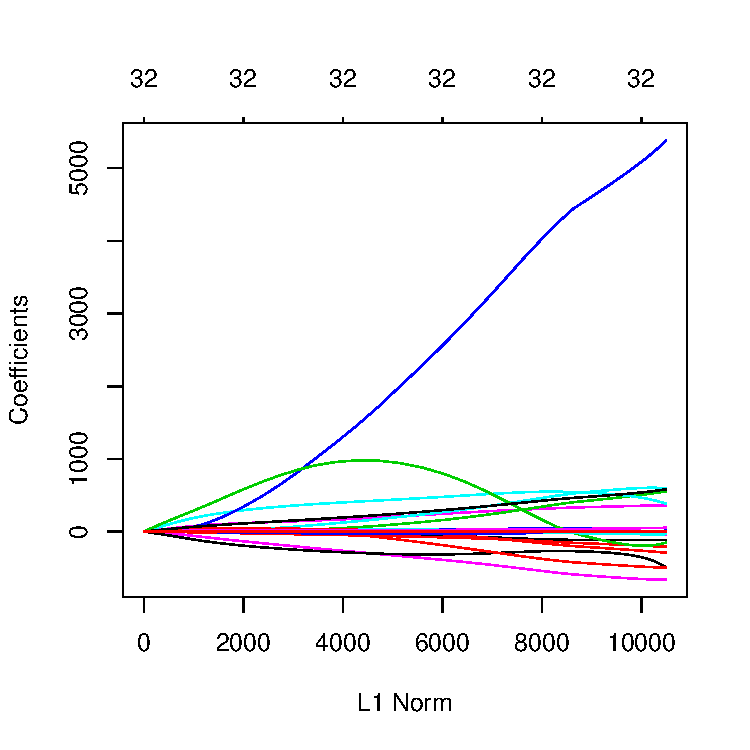
\includegraphics[width=0.8\linewidth]{Figures/ridge_model.pdf}
	\captionof{figure}{Coefficients $\beta_{j}$ against L1 Norm}
	\label{fig:ridge_model}
\end{center}

Each curve of the \ref{fig:ridge_model} corresponds to the ridge regression coefficient estimate for one of the 33 predictors, plotted as a function of $L1 Norm =$ . It is to be noted that the higher the L1 Norm, the closer to zero are the coefficients $\beta_{j}$.\\


In order to find the best tuning parameter $\lambda$ we perform a cross validation on the training data. \texttt{cv.glmnet} function runs a 10 fold cross validation on the data.

\begin{lstlisting}
model.ridge.cv.out = cv.glmnet(train_set.x, train_set.y,alpha=0)
plot(model.ridge.cv.out)
model.ridge.best.lambda = model.ridge.cv.out$lambda.min
\end{lstlisting}

\begin{center}
	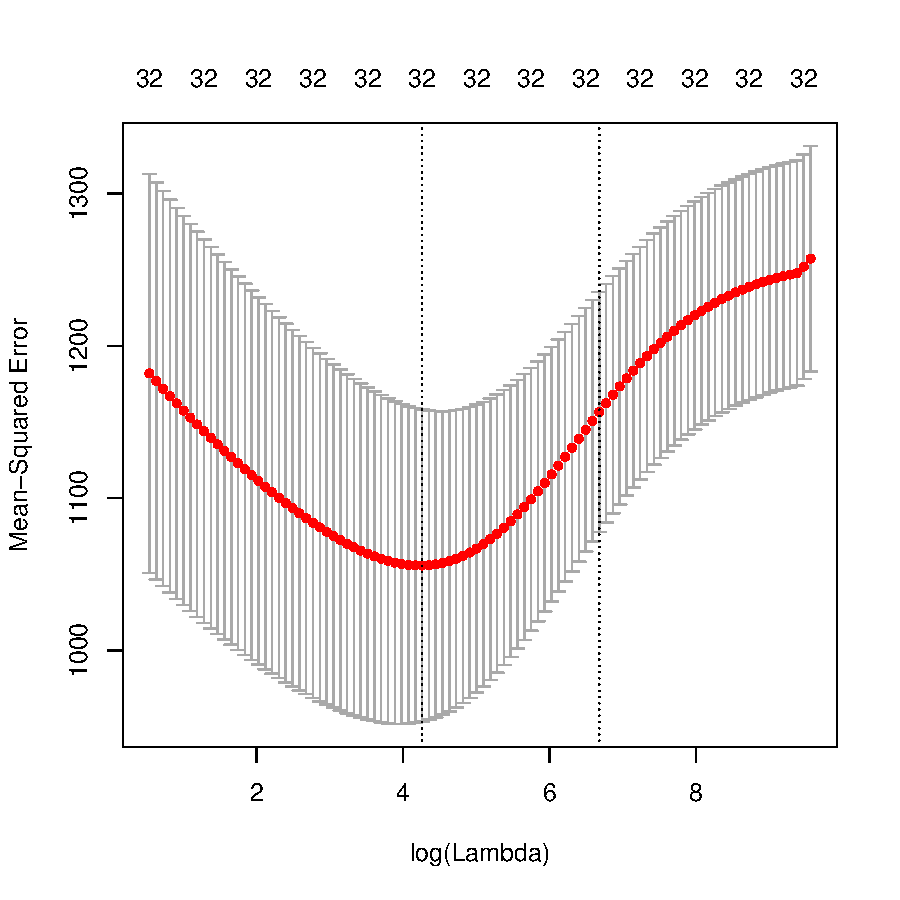
\includegraphics[width=0.8\linewidth]{Figures/cv_glmnet.pdf}
	\captionof{figure}{MSE against log($\lambda$)}
	\label{fig:cv_glmnet}
\end{center}

The value $\lambda$ that yields to the smallest MSE is shown in the graph \ref{fig:cv_glmnet} near $log(\lambda)=4$ and $log(\lambda)=5 $


\begin{lstlisting}
model.ridge.best = glmnet(train_set.x, train_set.y, lambda=model.ridge.best.lambda, alpha=0)
model.ridge.best.pred = predict(model.ridge.best, s=model.ridge.best.lambda, newx=test_set.x)

residuals = test_set.y - model.ridge.best.pred
errors = residuals^2
model.ridge.best.MSE = mean(errors)

plot(x=test_set.y, y=model.ridge.best.pred)
abline(0,1, col='red')

hist(residuals, freq=FALSE, main="Distribution of Residuals in Ridge")
residuals.mean = mean(residuals)
residuals.stdev = sqrt(var(residuals))
curve(dnorm(x, mean=residuals.mean, sd=residuals.stdev), col="darkblue", lwd=2, add=TRUE, yaxt="n")
\end{lstlisting}

\begin{center} 
	model.ridge.best.lambda = 45.07 \\
	model.ridge.best.MSE = 1063.3
\end{center} 

\begin{center}
	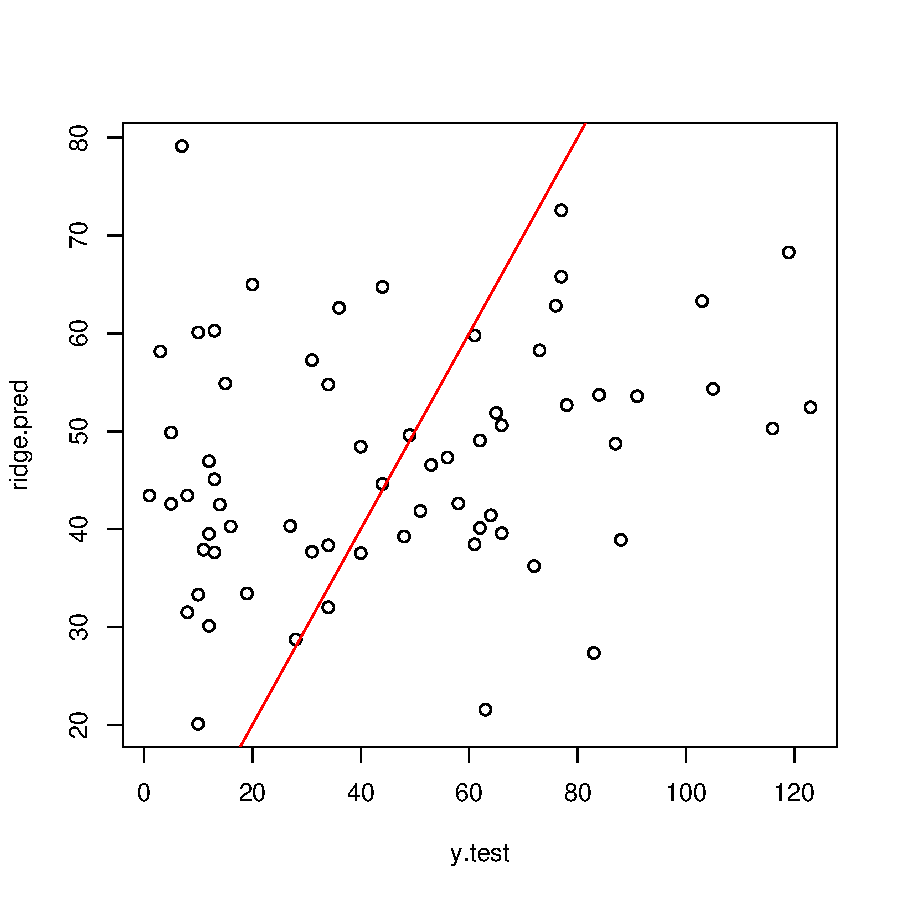
\includegraphics[width=0.8\linewidth]{Figures/ridge_yhat.pdf}
	\captionof{figure}{predicted Time $\hat{y}$ against real responses y }
	\label{fig:ridhe_yhat}
\end{center}

\begin{center}
	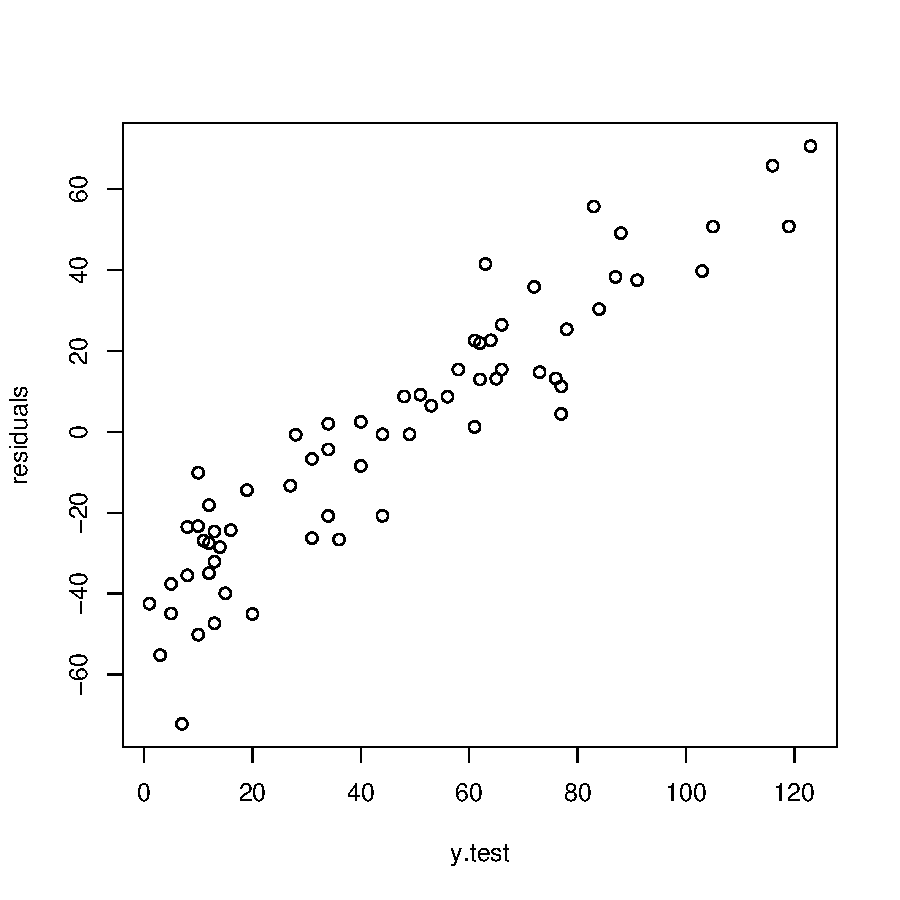
\includegraphics[width=0.8\linewidth]{Figures/ridge_resid.pdf}
	\captionof{figure}{Residuals against Time(y)}
	\label{fig:ridge_resid}
\end{center}

Performing a Ridge regression didn't really improve out MSE, we notice that we still have the same shape when we plot the predicted response against the real values. In fact we still have the extreme values scattered away from the line y=x while the values in the middle are grouped around it. The residuals shows most residuals are among -20 and 40, however we can't neglect the important number of observation that have residuals below -20.\\

After predicting the responses with the best\_$\lambda$,  we can also to get the coefficients $\beta_{j}$ for this model.

\begin{lstlisting}
predict(model.ridge, type="coefficients", s=model.ridge.best.lambda)[1:33,]
\end{lstlisting}

\begin{center}
	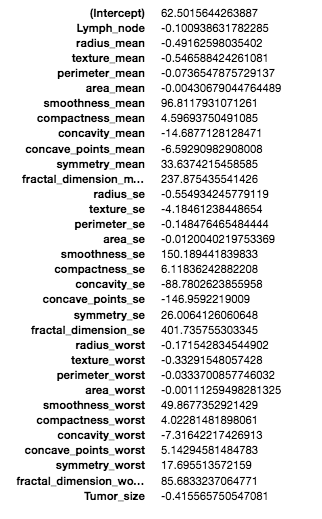
\includegraphics[width=0.8\linewidth]{Figures/ridge_coeff}
	\captionof{figure}{Ridge coefficients $\beta_{j}$ for ($\lambda$ = 45.07)}
\end{center}

\subsubsection{Model Analysis} \label{Ridge Model Analysis}
So we notice that some coefficients are very close to 0 such as \texttt{area\_se }(-0.012), but none of them is null. In fact Ridge Regression only shrinks the coefficients and does not perform any variable selection;  that is why we are going to use Lasso in the following part.

After comparing both MSE of the least squares (1285) and the Ridge Regression's one (1063) we notice that Ridge improves over Linear Regression. 
The question is how does Ridge improve over the least squares? It all can be summarized in\textbf{ biais-variance trade-off}. Let's take the following example where we we fit the model for each $\lambda$ and predict the responses for $\lambda\in[10^{-1},10^{4}]$. For each value of $\lambda$ we compute the MSE, the squared bias and the cube root of the variance. \textit{We computed the cube root in order to plot it with the bias in the same plot}.
\begin{lstlisting}
max = 100
biais2<-rep(0,max)
variance<-rep(0,max) 
mse<-rep(0,max)
grid=10^seq(4,-1, length=max)
for( i in 1:max)
{     
fit.ridge = glmnet(x.train, y.train, lambda=grid[i], alpha=0)
ridge.pred = predict(fit.ridge, s=grid[i] ,newx=x.test)
mse[i] = mean((ridge.pred - y.test)^2) #MSE
biais2[i] = (mean(ridge.pred - y.test))^2 #squared bias
variance[i] = (var(ridge.pred))^(1/3) #variance
}
plot(grid, variance,type='l', xlab="lambda", main="Biais-Variance trade-off")
lines(grid, biais2,col='red')
plot(MSE)
\end{lstlisting}

\begin{center}
	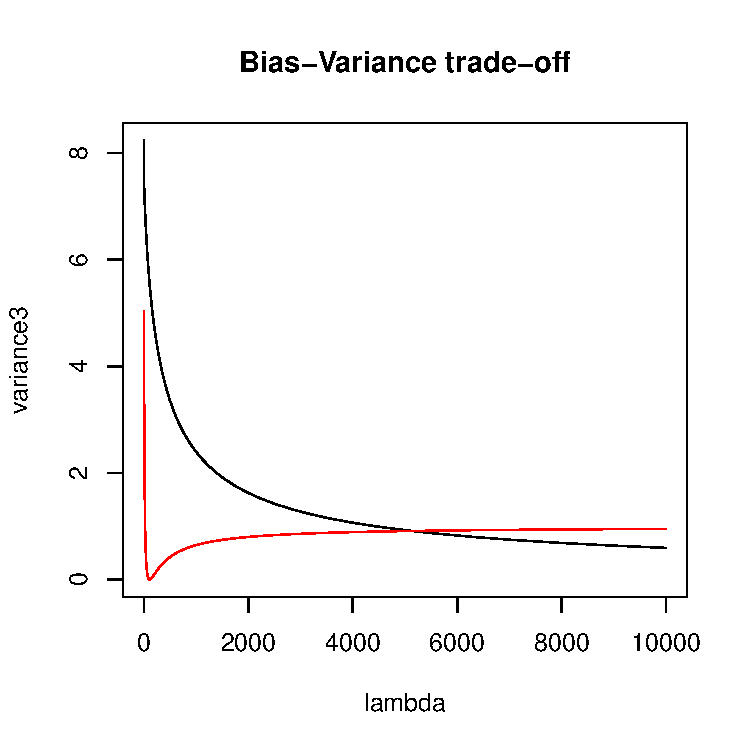
\includegraphics[width=0.8\linewidth]{Figures/ridge_bias_var.pdf}
	\captionof{figure}{Bias Variance trade-off, squared bias(red), root squared variance(black)}
\end{center}

\begin{center}
	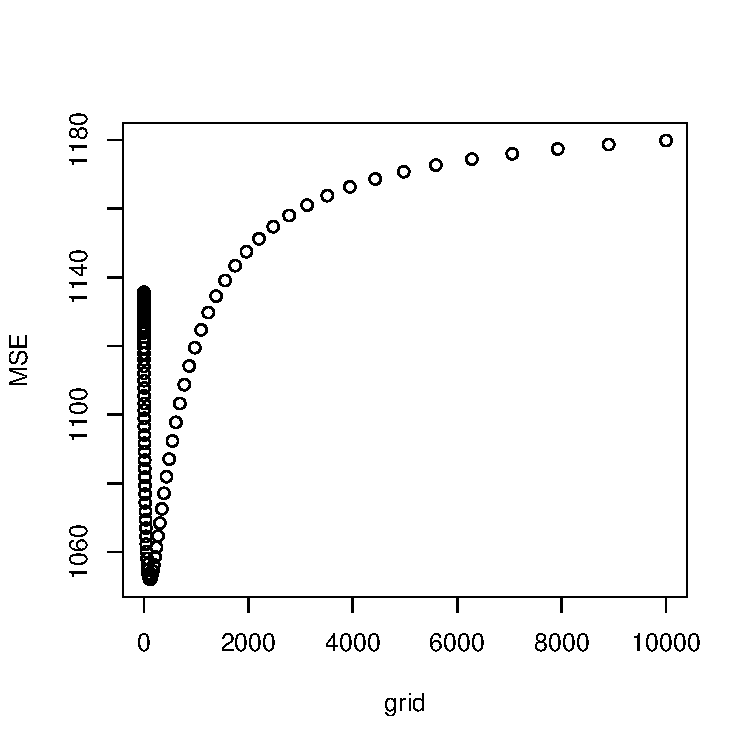
\includegraphics[width=0.8\linewidth]{Figures/ridge_mse.pdf}
	\captionof{figure}{MSE against $\lambda$}
\end{center}

At $\lambda=0$ (least squares), the variance is high but there is no bias.
As $\lambda$ increases the variance and bias decrease but at some point the variance continues to decrease while the bias starts increasing. Which means that the shrinkage of the coefficients by $\lambda$ reduces the variances on the expense of the bias, which can be explained by the fact that $\lambda$ in underestimating the coefficients by shrinking them. Let us compare now those results to the MSE curve. 
$$MSE = (E[\varTheta]-\varTheta)^{2} + Var(\varTheta) = (Bias[\varTheta])^{2} + Var(\varTheta)$$
Hence if the variance and the bias decrease significantly in the beginning the MSE will decrease too, and when the variance will decrease less and the bias will start increasing the MSE will increase too. We should also note that at at  $\lambda=0$ (least squares) the MSE is high.\\
To sum up, in linear regression we can have a low bias but a high variance, this is where the ridge regression improves over the least squares because it shrinks the variance on the expense of the bias.

\subsection{Lasso Regression}
As it was discussed on the previous section, Ridge regression's disadvantage is that it does not perform a variable selection. Lasso Regression however enables variable selection by minimizing the term:

\begin{equation} \label{eq2}
RSS + \lambda \sum_{j}{|\beta_{j}^{2}|}
\end{equation}	

The only difference with the term of Ridge is that we now have $|\beta_{j}^{2}|$ instead of $\beta_{j}^{2}$. This alternative will reduce the $\beta_{j}$ that are close to zero to null, hoping we have a more interpretable model with reducing the number of variables. To call the lasso model we use the same function \textbf{glmnet} but with the parameter \textbf{alpha=1}.

\subsubsection{Model Implementation}
\begin{lstlisting}
#Grid of 100 values of Lamba from 10^-2 to 10^10
grid = 10^seq(10,-2, length=100)
model.lasso = glmnet(train_set.x, train_set.y, alpha=1, lambda=grid)
plot(model.lasso)
\end{lstlisting}

\begin{center}
	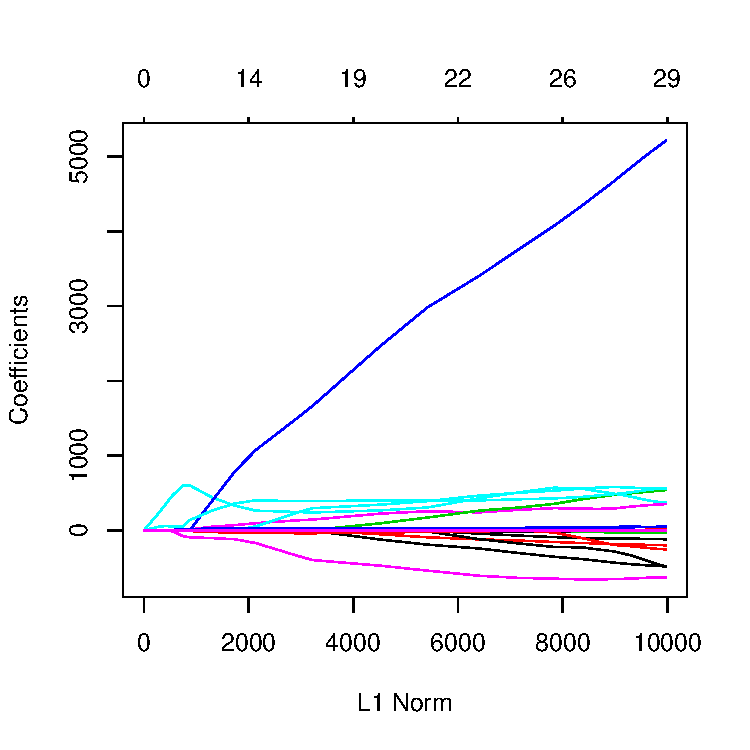
\includegraphics[width=0.8\linewidth]{Figures/lasso_model.pdf}
	\captionof{figure}{Coefficients against L1 Norm}
\end{center}

We notice that for some values of $\lambda$ the coefficients are null. We now perform the 10 fold cross validation on the training set to deduct the best tuning parameter. \textbf{cv.glmnet} does k-fold cross-validation for glmnet (by default k=10) it then  produces a plot and returns a value for lambda.

\begin{lstlisting}
model.lasso.cv.out = cv.glmnet(train_set.x, train_set.y, lambda=grid, alpha=1)
plot(model.lasso.cv.out)
model.lasso.best.lambda = model.lasso.cv.out$lambda.min
\end{lstlisting}

After running the cross validation we get the best lambda that minimized the term \ref{eq2}. We now can run a prediction on the test set with the best lambda and compute the residuals and the Test MSE.

\begin{lstlisting}
model.lasso.best = glmnet(train_set.x, train_set.y, lambda=model.lasso.best.lambda, alpha=1)
model.lasso.best.pred = predict(model.lasso.best, s=model.lasso.best.lambda, newx=test_set.x)

residuals = test_set.y - model.lasso.best.pred
errors    = residuals^2
model.lasso.MSE = mean(errors)

\end{lstlisting}

\begin{center}
	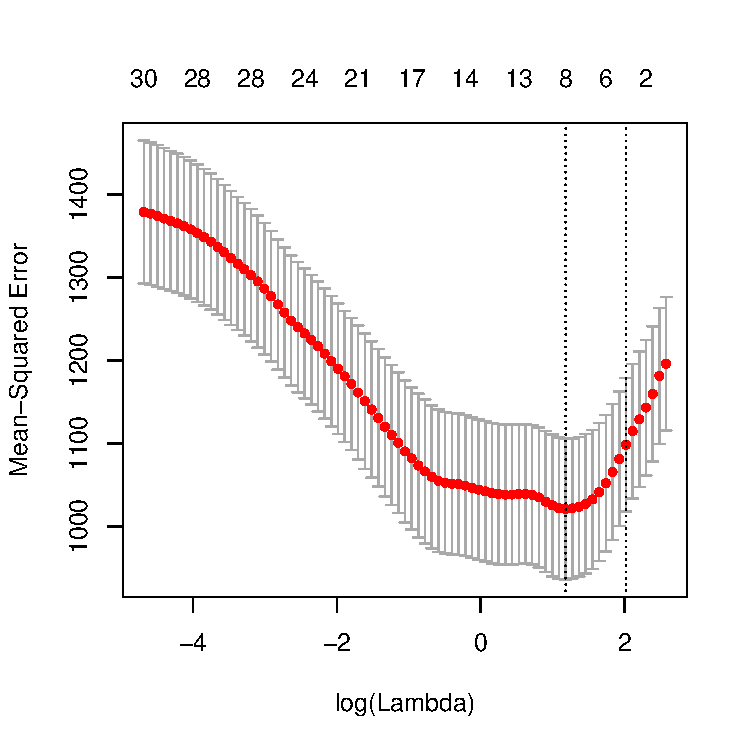
\includegraphics[width=0.8\linewidth]{Figures/lasso_mse.pdf}
	\captionof{figure}{MSE against $log(\lambda)$}
\end{center}

\begin{center} 
	model.lasso.best.lambda = 3.51 \\
	model.lasso.best.MSE    = 1045.92
\end{center} 

\begin{lstlisting}
# predicted values against real values
plot(x=test_set.y, y=model.lasso.pred)
#y = x
abline(0,1, col='red')

# histogram of residuals and the normal distribution
hist(residuals, freq=FALSE, main="Distribution of Residuals in Lasso")
residuals.mean = mean(residuals)
residuals.stdev = sqrt(var(residuals))
curve(dnorm(x, mean=residuals.mean, sd=residuals.stdev), col="darkblue", lwd=2, add=TRUE, yaxt="n")
dev.off()
\end{lstlisting}

\begin{center}
	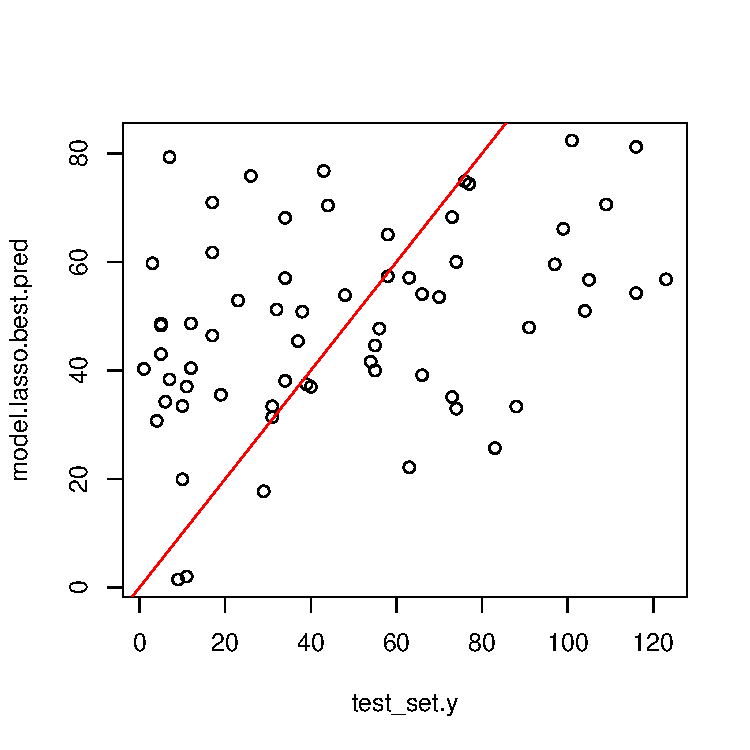
\includegraphics[width=0.8\linewidth]{Figures/lasso_predicted.pdf}
	\captionof{figure}{Predicted responses $\hat{y}$ against real values y}
\end{center}

\begin{center}
	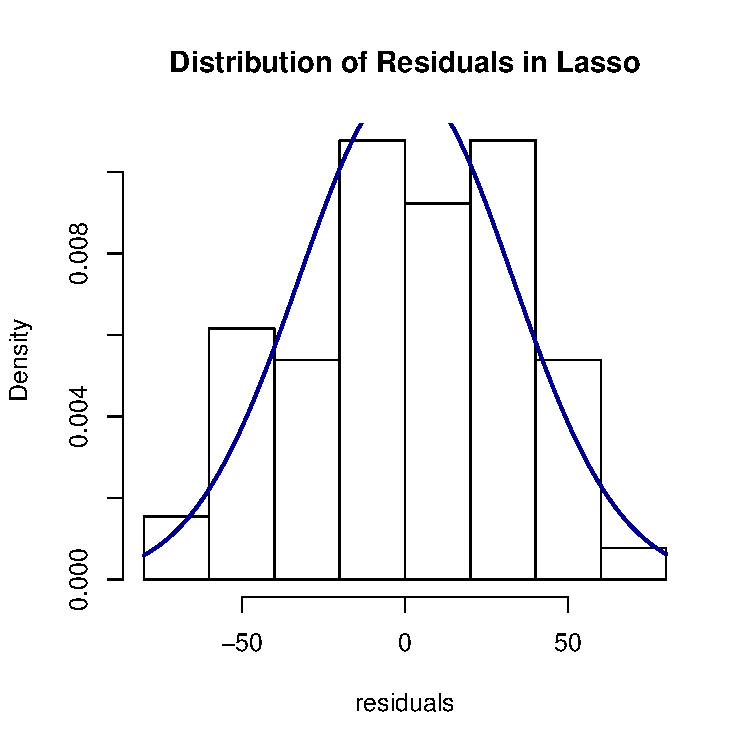
\includegraphics[width=0.8\linewidth]{Figures/lasso_residuals.pdf}
	\captionof{figure}{Distribution of Residuals in Lasso}
\end{center}

\begin{lstlisting}
predict(model.lasso, type="coefficients", s=model.lasso.best.lambda)[1:33,]
\end{lstlisting}

\begin{center}
	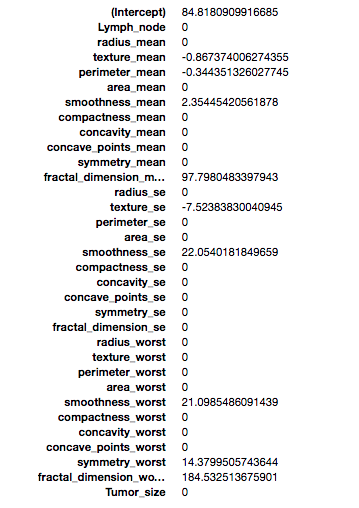
\includegraphics[width=0.8\linewidth]{Figures/lasso_coeff}
	\captionof{figure}{Lasso coefficients $\beta_{j}$ for ($\lambda$ = 3.25)}
\end{center}
We can clearly see that Lasso performed a variable selection by setting the unselected predictors' coefficients to 0

\subsubsection{Model Analysis}
 Lasso selected only 8 predictors out of 33 with a slightly improved test MSE compared to Ridge that uses all the predictors.Therefore we selected 25\% of variables The features selected to predict the Time are :
 \begin{itemize} 
 \item texture\_mean
 \item perimeter\_mean
 \item smoothness\_mean
 \item fractal\_dimension\_mean
 \item texture\_se
 \item smoothness\_se
 \item smoothness\_worst
 \item symmetry\_worst
 \item fractal\_dimension\_worst
\end{itemize}
Those are the features that with $\lambda = 3.25 $ their coefficients $\beta$ was not null .
Lasso selected only 10 predictors out of 33 with an slightly improved MSE compared to Ridge that uses all the 33 predictors.

\section{Linear Regression with Dimension Reduction}
\subsection{Idea}
In the Introduction, we mentioned the fact that some features are actually correlated. This means that they carry redundant information that make the model more complex, thus harder to fit. In this section, we will apply a Dimension Reduction method that decreases the number of features while keeping the information needed to predict \texttt{Time}.

Principal Component Analysis (PCA) is one such method. It consists in transforming the set of $p$ features into a set of $M$ orthogonal vectors ($M < p$) using linear transformations. The new set of vectors (called components) contains as much information as the initial set. "Information" is here defined in terms of variance, in other words, each new component should be able to explain as much variance as possible, while being orthogonal to the others.

Once a set of principal components is found, it can be used as an input to a simple linear regression to build what is called a Principal Component Regression (PCR) model. The number of components $M$ should be taken so that the model built with PCR has a minimum error value; once again, a 10 fold cross validation method can be used to determine the best $M$.

PCR is available in R with the package \texttt{pls} :
\begin{lstlisting}
library(pls)
model.pcr = pcr(Time ~ ., data=train_set, scale=TRUE, validation="CV")
\end{lstlisting}

We can then plot the MSE for each set of components :
\begin{lstlisting}
validationplot(model.pcr, val.type = "MSEP")
\end{lstlisting}

According to figure \ref{fig:pcr_cv}, the model with only 4 components yields to the lowest MSE. However, since $M = 4$ is found after running a random cross validation method, this number may be different if we run this algorithm another time.

\begin{figure}[!h]
	\centering
	\inputtikz{0.5}{Figures/pcr_cv.tex}
	\caption{PCR}
	\label{fig:pcr_cv}
\end{figure}

The function \texttt{summary} tells us that 4 components are enough to explain 75\% of the features' variance, which seems to be enough for this dataset. Indeed, this model performs better that the other linear regression methods : the MSE is approximatively equal to 967. 

\begin{figure}[!h]
	\centering
	\inputtikz{0.5}{Figures/pcr_hist.tex}
	\caption{PCR Raw Residuals Distribution}
	\label{fig:pcr_hist}
\end{figure}

\begin{figure}[!h]
	\centering
	\inputtikz{0.5}{Figures/pcr_predicted.tex}
	\caption{PCR Predicted values against Real values}
	\label{fig:pcr_predicted}
\end{figure}


\section{Models Comparaison}
\begin{tabular}{c c}
	Model & Mean Squared Error (MSE) \\
	KNN neighbours (with LOOCV) & 1146\\ 
	Linear Regression & 1285\\
	Best Subset	& 1067\\
	Ridge Regression & 1063 \\	
	Lasso & 1048\\
	PCR & 967 \\
\end{tabular}
\\We notice that the best MSE is found with the PCR model.
\begin{center}
	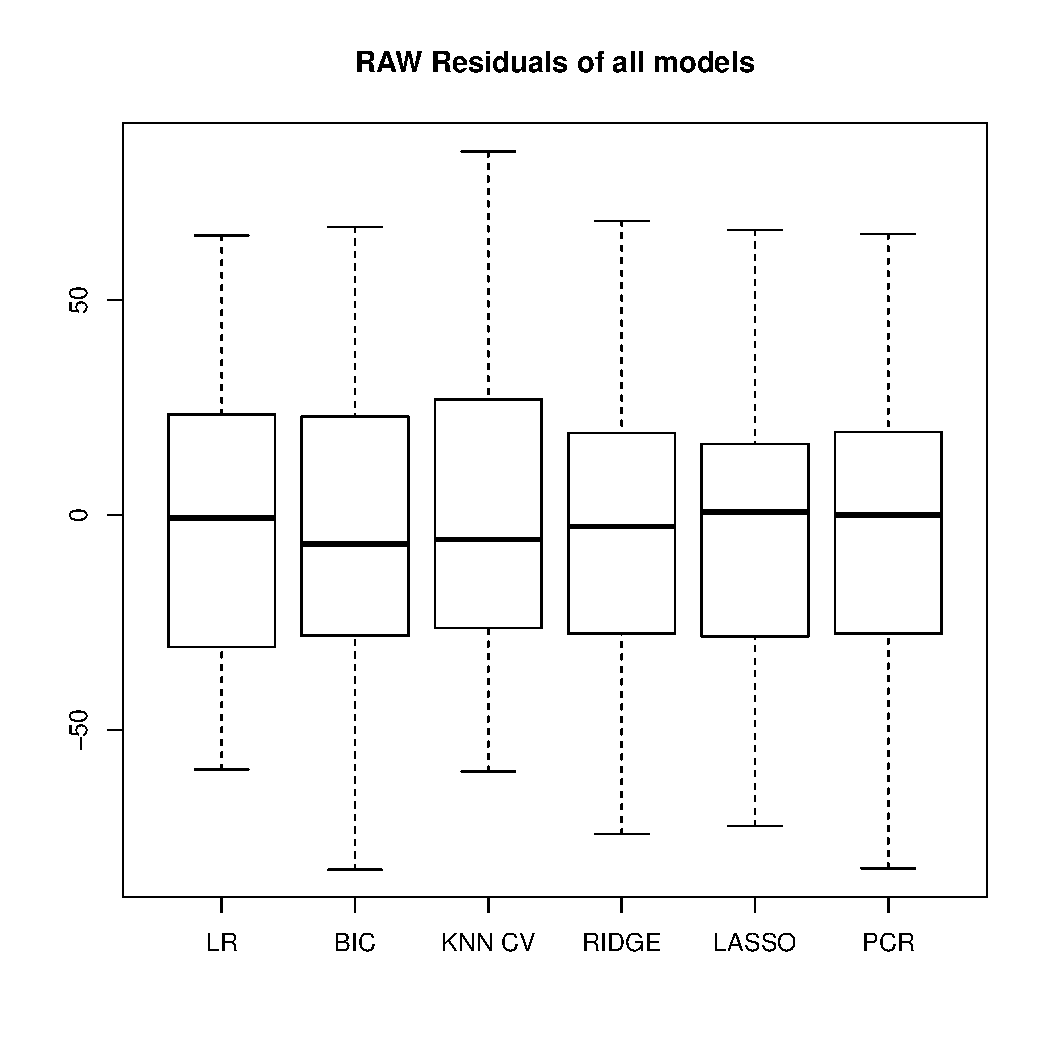
\includegraphics[width=0.8\linewidth]{Figures/all_resid.pdf}
	\captionof{figure}{BoxPlots of residuals off all models}
\end{center}

\subsection{KNN neighbors and Linear Regression}
 The linear regression is a \textbf{parametric method}, it comes with the hypothesis that there is a relationship between the response Y and the p predictors $X_{i}$ that can be expressed like $Y =\beta_{1}X_{1}+\beta_{2}X+{2}+...+\beta{p}X_{p}$. Their main advantages is that it is easy to use and to interpret however when the relationship between the predictors and the response is not linear the the results might not be satisfying. The KNN neighbors however is a non parametric method. In other words it makes no assumptions on the response Y. If we compare between the \textbf{test MSE} obtained by the KNN (1146) and the one obtained by the Linear Regression (1285), we see that the KNN does a better job. These arguments the fact that the model is not really linear. A remark that was made when observing the QQ plots in the first section. 
\subsection{Best subset Selection and Linear Regression Regularizations}
\subsubsection{Ridge \& Lasso }
The lasso's advantage over Ridge Regression is the variable selection; the model is thus easier to interpret. The MSE in Lasso is also slightly improved. In fact Lasso works better when there isn't an important number of predictors which corresponds to our case since we only have 33. In order to compare between their variance bias trade off. We run the ridge regression with all the different values of $\lambda$ but for Lasso we run the regression with the new data set that contains only 8 variables.\\ 
In order to create the new data\_set of 8 predictors we used the function \textbf{cbind} that binds columns and \textbf{data.frame} for storing data tables. cbind did not keep the columns'names so we renamed them using the function \textbf{colnames}.

\begin{lstlisting}
newdata_set =  data.frame(cbind(data_set$texture_mean, data_set$perimeter_mean, data_set$area_mean, 
data_set$fractal_dimension_mean,
data_set$texture_se, data_set$concavity_se, data_set$symmetry_worst, 
data_set$fractal_dimension_worst, data_set$Time))

colnames(newdata_set) <- c("texture_mean", "perimeter_mean", "area_mean", "fractal_dimension_mean", "texture_se",
"concavity_se","symmetry_worst", "fractal_dimension_worst", "Time" )

n 		= nrow(newdata_set)
p 		= ncol(newdata_set)
napp 	=  round(2*n/3)
ntst 	= n-napp
train 	= sample(1:n, napp)
newtrain_set 	= newdata_set[train,]
newtest_set 	= newdata_set[-train,]

newtrain_set.x = model.matrix(Time~.,newtrain_set)[,-1] 
newtrain_set.y = newtrain_set$Time
scale(newtrain_set.x, center = TRUE, scale = TRUE)

newtest_set.x =model.matrix(Time~., newtest_set)[,-1]
newtest_set.y = newtest_set$Time
scale(newtest_set.x, center = TRUE, scale = TRUE)
\end{lstlisting}

Now that we have our new data\_set, let's compare between the test MSE and variance bias trade off variance in function of the tuning parameter $\lambda$
\begin{lstlisting}
#Number of itterations
max         = 100
#Ridge: squared Biais, root square variance and MSE
biais2_r    = rep(0,max)
variance3_r = rep(0,max) 
MSE_r       = rep(0,max)

#Lasso: squared Biais, root square variance and MSE
biais2_l    = rep(0,max)
variance3_l = rep(0,max) 
MSE_l       = rep(0,max)

#Grid of lamba between 10^-1 and 10^4
grid        = 10^seq(4,-1, length=max)
for( i in 1:max)
{    
	# Ridge Regression
	model.ridge = glmnet(train_set.x, train_set.y, lambda=grid[i], alpha=0)
	model.ridge.pred = predict(model.ridge, s=grid[i] ,newx=test_set.x)    
	MSE_r[i] = mean((model.ridge.pred - test_set.y)^2) #MSE
	biais2_r[i] = (mean(model.ridge.pred - test_set.y))^2 #squared bias
	variance3_r[i] = (var(model.ridge.pred))^(1/3) #sqrt cubic of variance

	#Lasso Regression with 8 predictors
	model.lasso = glmnet(newtrain_set.x , newtrain_set.y, lambda=grid[i], alpha=1)
	model.lasso.pred = predict(model.lasso, s=grid[i], newx=newtest_set.x) 
	MSE_l[i] = mean((model.lasso.pred - test_set.y)^2) #MSE
	biais2_l[i] = (mean(model.lasso.pred - test_set.y))^2 #squared bias
	variance3_l[i] = (var(model.lasso.pred))^(1/3) #sqrt cubic of variance   
}
#Red for Ridge
#Variance
plot(grid,variance3_r,type="l", xlab="lambda", ylab="root squared Var and squared Biais",col="red",ylim=range(biais2_r, variance3_r, biais2_l, variance3_l), 		main="Bias(dashed)-Variance(line) trade-off of Ridge(Red) and Lasso(Blue)") 
#Biais
lines(grid,biais2_r,col="red", lty=2)
 
#Blue for Lasso
#Variance
lines(grid,variance3_l,col="blue")
#Biais 
lines(grid,biais2_l,col="blue",lty=2) 
\end{lstlisting}


\begin{center}
	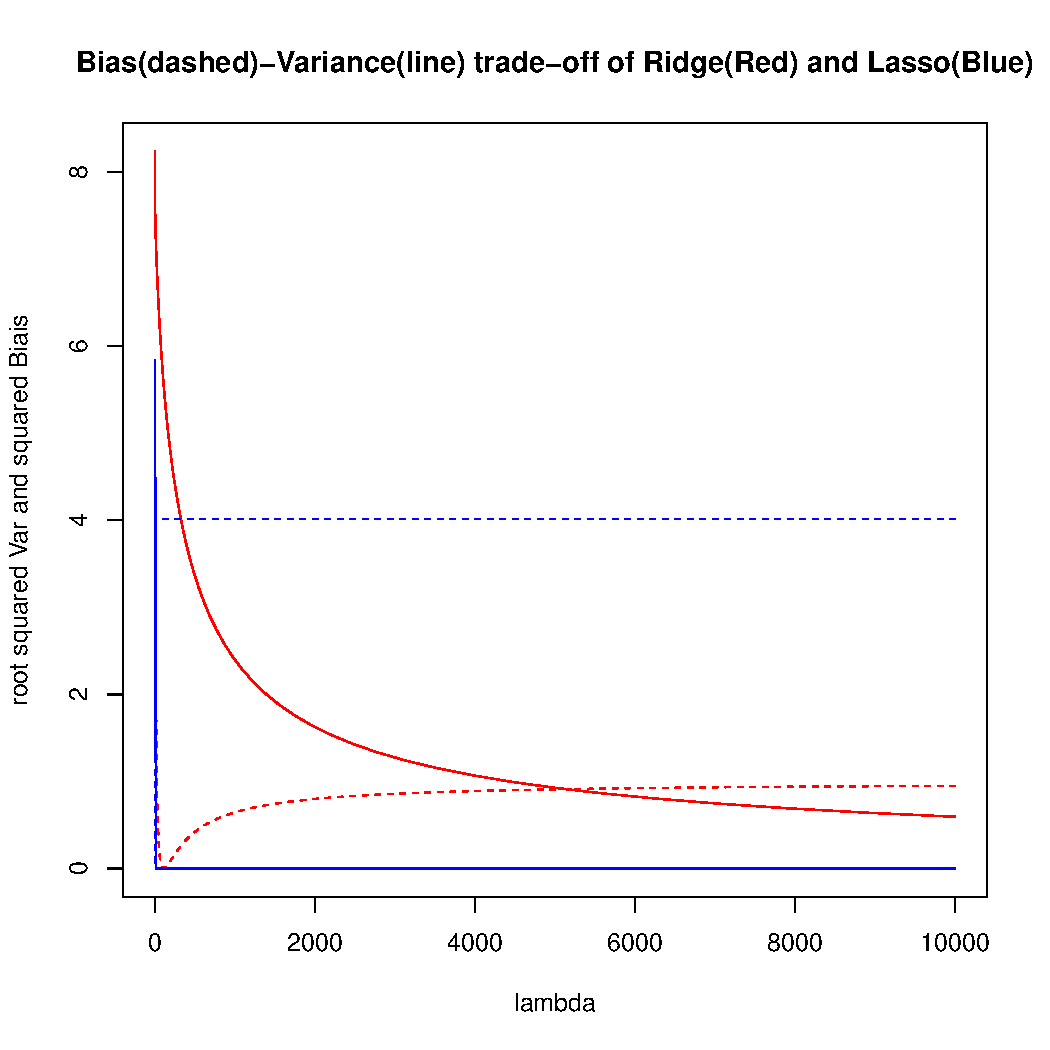
\includegraphics[width=0.8\linewidth]{Figures/var_biais_ridge_lasso.pdf}
	\captionof{figure}{Bias(dashed line)-Variance(line) Trade off of Ridge(Red) and Lasso(Blue)}
\end{center}
As it was stated in the subsection above \ref{Ridge Model Analysis} both Ridge and Lasso influence on the bias and the variance same way.
It is clear from the curves above that Lasso decreases the variance more on the expense of the bias which explains why the Ridge's vaiance is higher than the Lasso's one but its bias is smaller. \\
These leads us to conclude that neither of the models performs better than the other. Lasso will be more pertinent to use if we have few predictors as it will set some coefficients to null and so the model will be easier to interpret. Nevertheless if we have lot of predictors Ridge might be a better idea because all the coefficients will be small. 

\subsubsection{Regularization \& Best subset}
Both Lasso and Best Subset perform a variable selection, their MSE are close but with the Best Subset we only kept 3 variable which is 38\% less predictors. How can we compare between those two approaches?\\
First Lasso adds up a new tuning parameter to penalize the coefficients which is why it is named shrinkage method. In contrast to the Best subset selection that doesn't add up anything. Therefore the regression coefficients obtained by Lasso are biased.
\subsection{Dimension Reduction}



\chapter{Phoneme Recognition}
\section{Context}
In the context of speech recognition the aim is to predict which of the phonemes is pronounced by the subject. In this case, we have five phonemes to recognize :\\ 
\begin{center}
	$g = \left\{
	\begin{array}{l}
	\textbf{"sh"} \text{ as in } "she" \\
	\textbf{"dcl"} \text{ as in } "dark" \\
	\textbf{"iy"} \text{ as the vowel in } "she" \\ 
	\textbf{"aa"} \text{ as the vowel in }  "dark"\\
	\textbf{"ao"} \text{ as the first vowel in }  "water"
	\end{array}
	\right.$
\end{center}

\section{Dataset Description}

The study involved 4509 speeches pronounced by 50 male speakers. The method used for speech recognition is the Log-periodogram, an estimate of the spectral density of the sound signal.

Our dataset is composed of 4509 log-periodograms (observations) of length 256 (features). The column labelled \texttt{speakers} identifies the different speakers. We notice that some are labeled train and some test. Hence we have a training set composed of 3340 observations (74\%) and a test set that comprises 1169 observations (26\%). The column \texttt{g} shows the responses. The frequencies of each phoneme for the 4509 speeches are shown in the table below.

\begin{center}
\begin{tabular}{l c c c c c}
 Phonemes	 & aa &  ao & dcl & iy & sh \\
Train & 519 & 759 & 562 & 852 & 648\\
Test  & 176 & 263 & 195 & 311 & 224\\
Total & 695 & 1022 & 757 & 1163 & 872
\end{tabular}
\captionof{table}{Frequencies of phonemes in the train and test data set}
\end{center}

Our dataset tells us which speaker the periodogram is extracted from. We could input this information in the model, however, the system may not be aware of the speaker in a real-case scenario, therefore, we will not consider the speaker as a feature. 

\begin{lstlisting}
data_set = read.csv("phoneme.data.txt")
head(data_set)
data_set.nb_features = 256
\end{lstlisting}

\section{Measure to Compare Models}
Before building any model, we have to properly define the measures we will use later to compare their performance. In a classification problem, "accuracy" is often used. It is defined by :
$$
	A = \frac{\text{Number of Good Predictions}}{\text{Number of Cases}}
$$

This is a very simple measure that may cause some issues when applied on classification problems that deal with skewed classes. For instance, let $A$ and $B$, two classes. $A$ contains 95\% of the dataset, while $B$ contains the remaining 5\%. Let $M$ a pretty bad classifier which classifies the whole dataset in class $A$. According to the definition stated above, this classifier has an accuracy of 95\%, which is excellent. In this case, more specific performance measures have to be applied.

However, our current classification problem do not deal with skewed class since all classes are almost equally-represented in the dataset. Therefore, we will be able to run this performance measure without any important issue. This measure will be aplied on the test set in order not to include any biais.

\begin{lstlisting}
train_set= data_set[1:3340, 2:258]
train_set.x = train_set[,1:256]
train_set.y = train_set[,257]

test_set = data_set[3341:4509, 2:258]
test_set.x = test_set[,1:256]
test_set.y = test_set[,257]
\end{lstlisting}

\section{Classification}

\subsection{LDA - Linear Discriminant Analysis}
The first model we are going to use takes advantage of Bayes' Theorem. Let $f_k(x)$ the class-conditional density of $X$ when $Y=k$, and $\pi_k$ the prior probability of class $k$. Bayes' Theorem proposes the following statement : 

$$
\mathbb{P}(Y = k | X = x) = \frac{f_k(x)\pi_k}{\sum_{l = 1}^{K}f_l\pi_l} 
$$

$X$ belongs to the class whose conditional probability is the highest.

If the class distribution of the dataset is representative of the real distribution, we can estimate $\pi_k$ by calculating the proportion of $k$ class elements in the dataset. How can we now estimate $f_k(x)$ ? Linear Discriminant Analysis assumes that all $f_k(x)$ are Gaussian distributions whose covariance matrix $\Sigma$ are the same.

\subsubsection{Model Implementation}
The function \texttt{lda} works the same was as \texttt{lm} for linear regression. It returns the group means that are the average of each predictor in each class. The coefficients of linear discriminants output are used to form the LDA decision rule. The prior probability is the percentage of the response for each class in the observation.

\begin{lstlisting}
library(MASS)
model.lda = lda(g ~ ., data=train_set)
summary(model.lda)
\end{lstlisting}

\begin{verbatim}
Prior probabilities of groups:
aa         ao         dcl        iy         sh 
0.1553892  0.2272455  0.1682635  0.2550898  0.1940120 
\end{verbatim}

The prior probabilities tell us that in the train observation 15\% of phonemes are \texttt{aa} , 23\% \texttt{ao}, 17\% \texttt{dcl}, 25\% \texttt{iy} and 19\% \texttt{sh}.

Now that we trained the model we can call the \texttt{predict} function to predict the responses of the test set of data. This function returns an element \texttt{class}, a list of the predicted phonemes. An element \texttt{posterior} with the posterior probability of the response of the $k$-th class.  Last the linear discriminants are found in \texttt{x}.

\begin{lstlisting}
model.lda.predicted = predict(model.lda,newdata=test_set)
perf = table(test_set$g,model.lda.predicted$class)
perf
sum(diag(perf))/dim(test_set)[1]
\end{lstlisting}

The table perf of the predicted responses is shown below:
\begin{center}
\begin{verbatim}
 g 	 aa  ao dcl  iy  sh
aa  129  47   0   0   0
ao   39 223   0   1   0
dcl   0   0 190   5   0
iy    0   0   2 309   0
sh    0   0   0   0 224

0.919589392643285
\end{verbatim}
\end{center}

Here is an example of how this table is read, for the second line
when the phoneme pronounced is \texttt{aa} , the speech recognition detects that 129 is detected as \texttt{aa} and 47 as \texttt{ao}, in other words only 27\% is misclassified.
In order to compute the total error rate we divide the sum of the diagonal terms (which are the true phonemes detected) and divide it by the number total of observations We find that in 92\% of the cases the speech recognition detected right the phoneme. This classifier performs quite well, but it does not work well with the phonemes \texttt{aa} and \texttt{ao} which sound very similar.

\subsubsection{Improvements with PCA}
The dataset has a high number of features (256) that may prevent the model from fitting well. We can cope with this performance issue by applying a dimension reduction method, such as Principal Component Analysis (PCA). The function\texttt{prcomp} is available in R to compute the principal components of the 256 features. Since PCA depends on the scaling of the inputs, it is important to scale and center each feature.
\begin{lstlisting}
pca = prcomp(train_set.x, center = TRUE, scale. = TRUE)
\end{lstlisting}

The main question is now : how many principal components should we use to replace our main features ? The best number of components $M$ yields to the highest accuracy. The following code finds the best $M$ for the test set.

\begin{lstlisting}
accs = matrix(0, 50, 1)

for (M in 2:50) {
	train_set.pca.x = as.data.frame(pca$x[,1:M])
	train_set.pca = as.data.frame(cbind(train_set.y, train_set.pca.x))
	
	test_set.pca.x = predict(pca, newdata = test_set.x)[,1:M]
	test_set.pca = as.data.frame(cbind(test_set.y, test_set.pca.x))
	
	model.lda.pca = lda(train_set.y ~ ., data = train_set.pca)
	model.lda.pca.predicted = predict(model.lda.pca,newdata=test_set.pca)
	
	perf = table(test_set$g,model.lda.pca.predicted$class)
	accs[M] = sum(diag(perf))/dim(test_set)[1]
}

which.max(accs[-1])
plot(accs[-1])
\end{lstlisting}

\begin{figure}[!hb]
	\centering
	\inputtikz{0.5}{Figures/lda_pca.tex}
	\caption{Best $M$ for LDA + PCA on Test Set}
	\label{fig:lda_pca}
\end{figure}

The best $M$ on the test set is 8 (figure \ref{fig:lda_pca}), which yields to an accuracy of 92.2\%.

\begin{verbatim}
g    aa  ao dcl  iy  sh
aa  131  45   0   0   0
ao   40 223   0   0   0
dcl   0   0 191   4   0
iy    0   0   1 309   1
sh    0   0   0   0 224
\end{verbatim}

 However, this method raises a biais since we computed $M$ based on the test set. A proper way to find $M$ is using a k fold cross validation technique on the training set. The following code aims to find the best $M$ in the range $[2:50]$.

\begin{lstlisting}
library(caret)

accs = matrix(0, 50, 1)
for (M in 2:50) {
	a.train_set.pca.x = as.data.frame(pca$x[,1:M])
	a.train_set.pca = as.data.frame(cbind(train_set.y, a.train_set.pca.x))
	
	folds = createFolds(train_set.pca$train_set.y)
	
	acc = 0;
	for (k in 1:10) {
		validation_indexes = folds[[k]]
		a.train_set.x = a.train_set.pca.x[-validation_indexes,]
		a.train_set = a.train_set.pca[-validation_indexes,]
		
		a.validation_set.x = a.train_set.pca.x[validation_indexes,]
		a.validation_set = a.train_set.pca[validation_indexes,]
		
		model.lda.pca = lda(a.train_set$train_set.y ~ ., data = a.train_set)
		model.lda.pca.predicted = predict(model.lda.pca,newdata=a.validation_set)
		
		perf = table(a.validation_set$train_set.y,model.lda.pca.predicted$class)
		acc = acc + sum(diag(perf))/dim(a.validation_set)[1]
	}

	acc = acc / 10
	accs[M] = acc
}
\end{lstlisting}

\begin{figure}[!hb]
	\centering
	\inputtikz{0.5}{Figures/lda_pca_cv.tex}
	\caption{Best $M$ for LDA + PCA on Training Set with Cross Validation}
	\label{fig:lda_pca_cv}
\end{figure}

According to the graph shown in figure \ref{fig:lda_pca_cv}, the best $M$ is 42, which yields to an accuracy score of 92.04\% :
\begin{verbatim}
g    aa  ao dcl  iy  sh
aa  129  47   0   0   0
ao   39 224   0   0   0
dcl   0   0 189   6   0
iy    0   0   1 310   0
sh    0   0   0   0 224
\end{verbatim}

\subsection{QDA - Quadratic Discriminant Analysis}
This method is very similar to the LDA, the only difference being that the covariance matrices $\Sigma_k$ are not necessarily equal.

\subsubsection{Model Implementation}
In R, the function \texttt{qda} creates a classifier based on the QDA methods. It works the same way as \texttt{lda} :
\begin{lstlisting}
model.qda = qda(g ~ ., data=train_set)
\end{lstlisting}

\begin{verbatim}
g    aa  ao dcl  iy  sh
aa   27 143   0   3   3
ao    2 259   0   1   1
dcl   0   0 165  29   1
iy    0   0   0 311   0
sh    0   0   1   1 222
\end{verbatim}

This model performs worse than the LDA : the accuracy is about 84.2\%. It does not manage to make the difference between class \texttt{aa} and \texttt{ao}. This may mean that the covariance matrices $\Sigma_k$ are almost equal and that we will not be able to make this model more accurate than LDA.

\subsubsection{Improvements with PCA}
We know that the error rate of QDA highly depends on the size of the dataset and the number of features. Therefore, we may be able to improve its performance using PCA using the same 10 fold cross validation technique we used earlier.

\begin{figure}[!hb]
	\centering
	\inputtikz{0.5}{Figures/qda_pca_cv.tex}
	\caption{Best $M$ for QDA + PCA on Training Set with Cross Validation}
	\label{fig:qda_pca_cv}
\end{figure}

In this case, the algorithm returns $M = 12$ (figure \ref{fig:qda_pca_cv}) which leads to 92\% accuracy. We successfully improved QDA's performance but the accuracy is still not better than LDA, as expected.

\begin{verbatim}
g    aa  ao dcl  iy  sh
aa  124  52   0   0   0
ao   35 228   0   0   0
dcl   0   0 192   3   0
iy    0   0   2 308   1
sh    0   0   0   0 224
\end{verbatim}

\subsection{Logistic Regression}

Logistic Regression is a type of Linear Classification method that models the posterior probabilities with linear functions. When there are only two features to deal with, the model is definined by : 

$$
\log \frac{\mathbb{P}(Y = 0 | X = x)}{\mathbb{P}(Y = 1 | X = x)} = \beta_0 + \beta x
$$

If $\beta_0 + \beta x$ is positive, $Y$ is most likely to be equal to 0; otherwise, $Y$ is most likely to be equal to 1.  \\

In a multinomial scenario, like our case, more complex methods have to be applied. In particular, the library \texttt{nnet} provides us with a function called \texttt{multinom} that uses a feedforward Neural Network with a single hidden layer to fit a multinomial logistic regression model. This kind of Neural Networks often runs a backpropagation method along with an iterative optimization algorithm to estimate the weights of each neuron. That is why we have to specify the maximum number of iterations.

\begin{lstlisting}
library("nnet")
model.lr = multinom(formula = g ~ . , data=train, MaxNWts=2000, maxit=1000)
\end{lstlisting}

\begin{lstlisting}
model.lr.predicted = predict(model.lr,newdata=test_set)
perf = table(test_set$g,model.lr.predicted)
perf
sum(diag(perf))/dim(test_set)[1]
\end{lstlisting}

Neural Networks are known to be quite long to train, that is why it takes several seconds to fit the model. The error rate is similar to QDA (accuracy is about 86\%), however it performs better on \texttt{aa} and \texttt{ao}: 
\begin{verbatim}
g    aa  ao dcl  iy  sh
aa  114  54   4   2   2
ao   47 197   8  10   1
dcl   0   1 192   2   0
iy    0   2  12 292   5
sh    0   1   6   1 216
\end{verbatim}

\subsubsection{Improvements with PCA}
Once again, we can use PCA to reduce the input dimension in order to make the neural network fit better and faster. However, since \texttt{multinom} runs significantly slower than the other methods, we will only find the best $M$ in the range $[2, 20]$ using a 5 fold cross validation method.

\begin{figure}[!hb]
	\centering
	\inputtikz{0.5}{Figures/lr_pca_cv.tex}
	\caption{Best $M$ for LR + PCA on Training Set with Cross Validation}
	\label{fig:lr_pca_cv}
\end{figure}

The best accuracy is reached at $M = 17$, accuracy on the test set being approximatively 91\% : 
\begin{verbatim}
g    aa  ao dcl  iy  sh
aa  122  54   0   0   0
ao   34 228   0   1   0
dcl   0   0 190   5   0
iy    0   4   3 303   1
sh    1   0   1   1 221
\end{verbatim}

\section{Models Comparison}

According to our comparison measure (accuracy), the best model we found is LDA with PCA. LDA is the most interesting model so far because of its simplicity and its performance with and without PCA transformation. QDA and LR does not perform well with the full set of features, but they are as good as LDA when a PCA feature subset selection is applied.  

\end{document}
